\subsection{Телескоп}
\term{Телескоп}~--- устройство для наблюдения удаленных объектов. На данный момент существуют телескопы  для наблюдения во всех  диапазонах электро-магнитного излучения. По наблюдаемому диапазону телескопы делят на \imp{оптические} телескопы, \imp{радиотелескопы}, \imp{рентгеновские} телескопы и \imp{гамма-те\-ле\-скопы}. Каждый из классов в свою очередь содержит множество подклассов. Поговорим подробнее про оптические телескопы.

Оптические телескопы по своей схеме делятся на три типа: \imp{рефлекторы} (диоптрические), \imp{рефракторы} (катаптрические) и \imp{катадиоптрические}.

\vspace{-.3pc}
\begin{figure}[h!]
	\centering
	\begin{subfigure}{0.49\tw}
		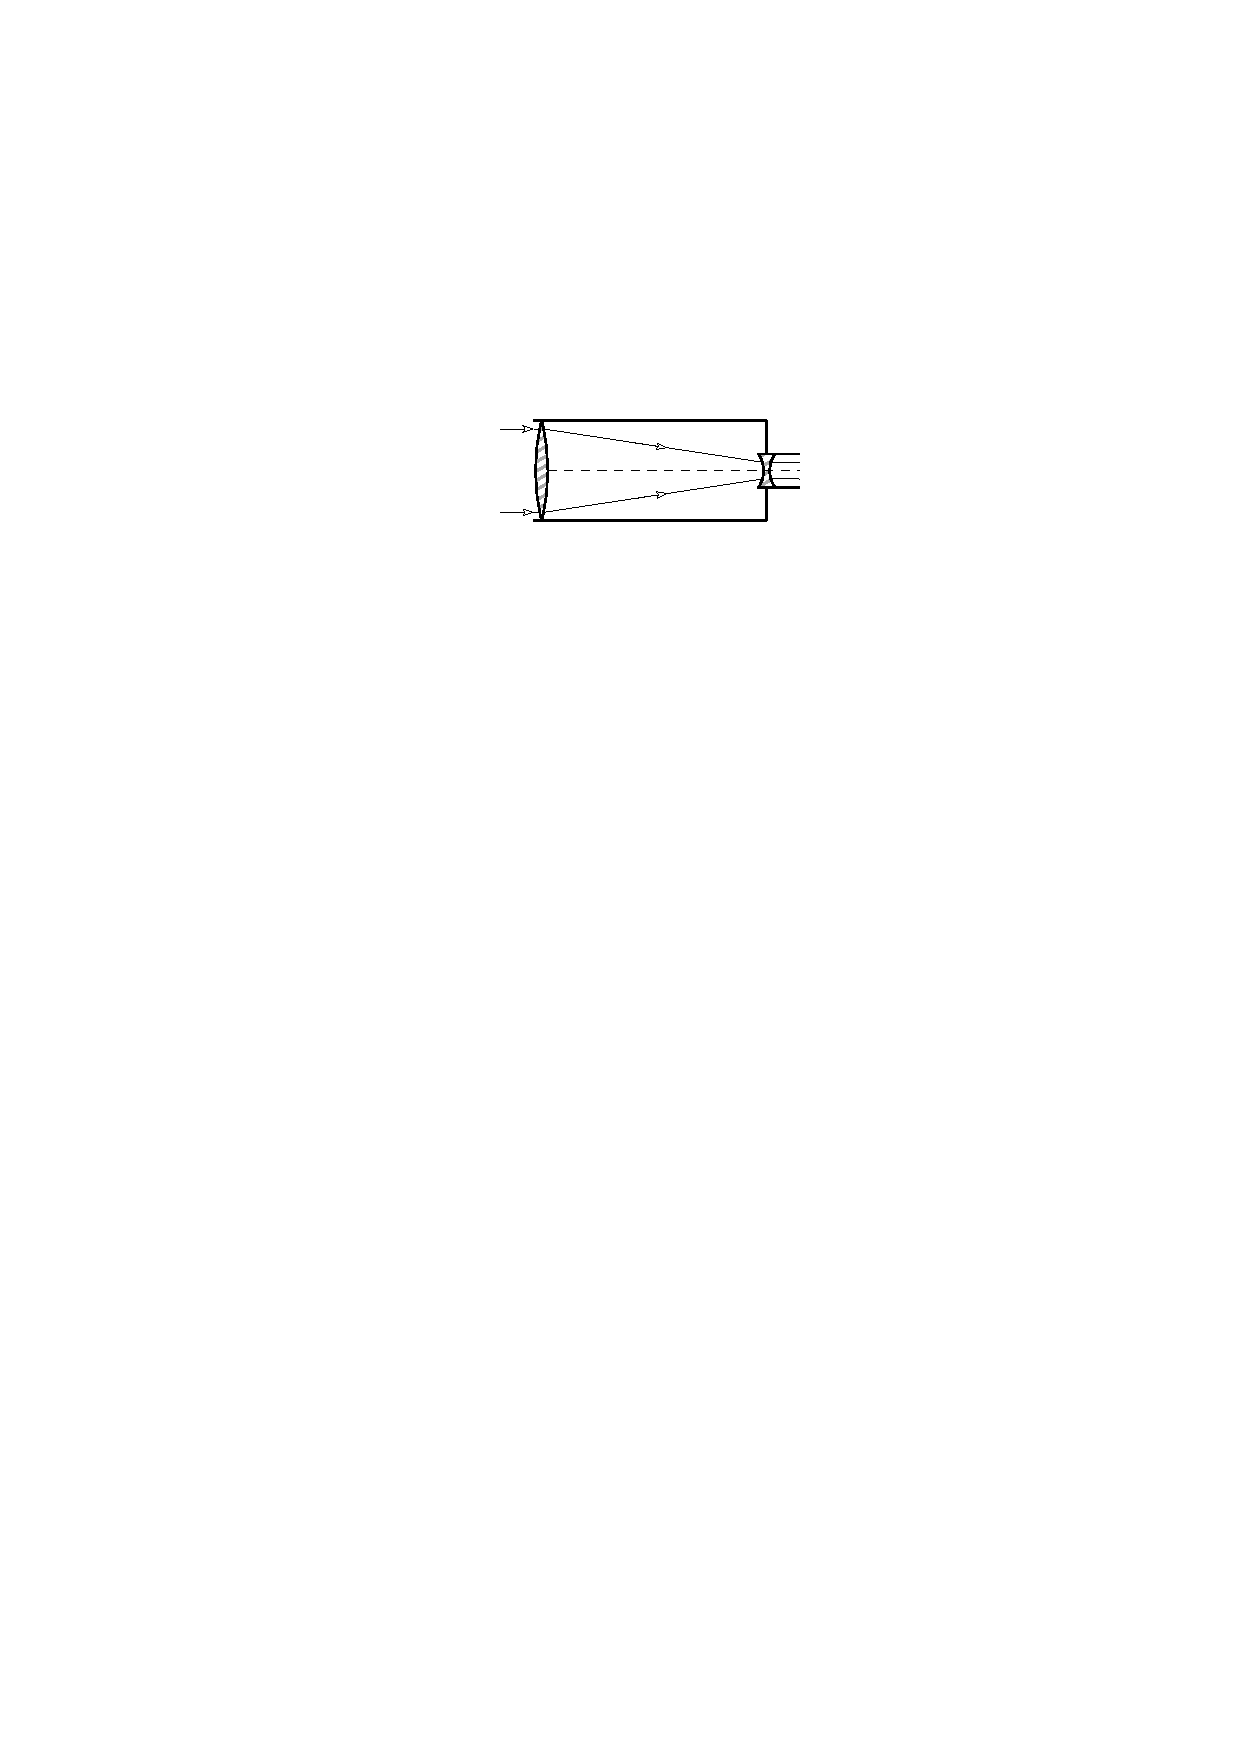
\includegraphics[width = \tw]{Galiley}
		\caption{Рефрактор системы Галилея}
	\end{subfigure}
	\hfill
	\begin{subfigure}{0.49\tw}
		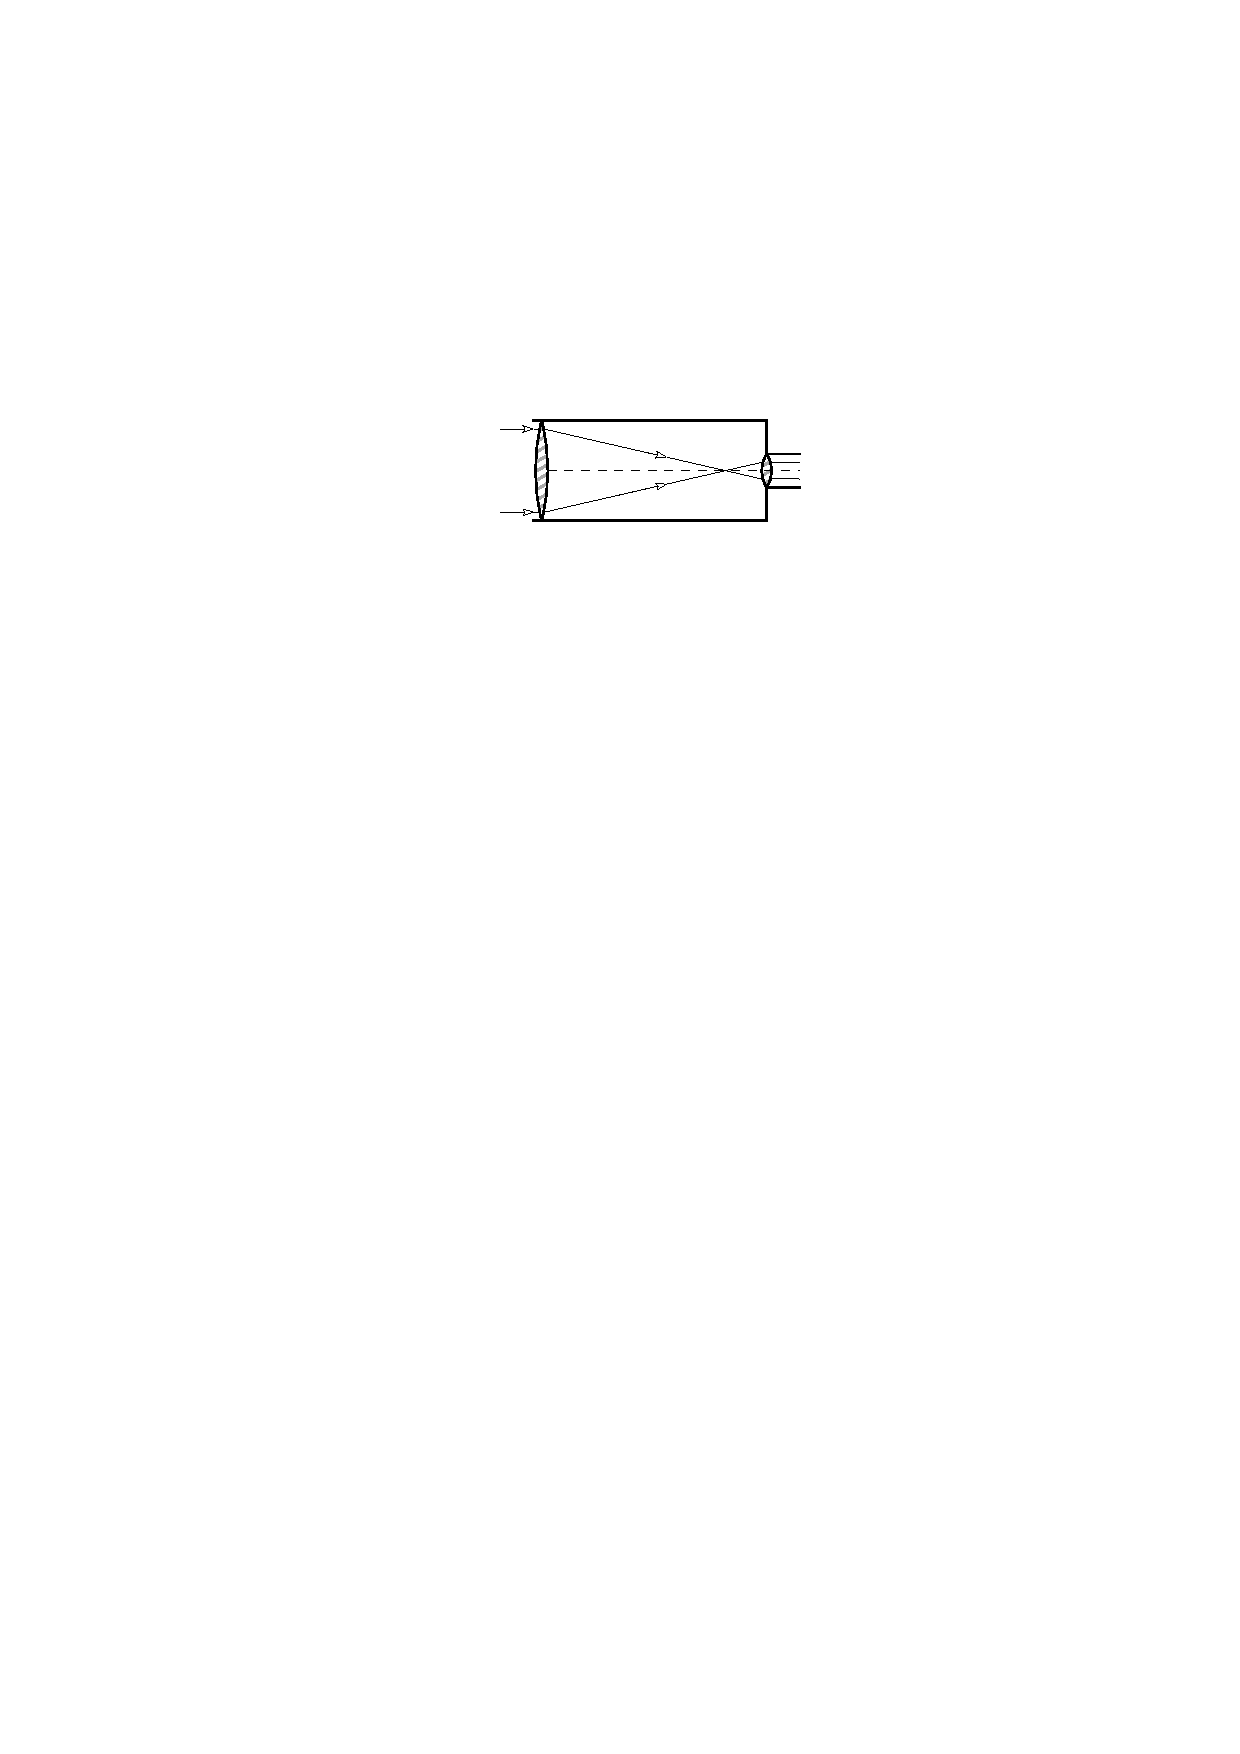
\includegraphics[width = \tw]{Kepler}
		\caption{Рефрактор системы Кеплера}
		\label{Kepler}
	\end{subfigure}
	\caption{Оптические схемы телескопов рефракторов}
\end{figure}
\term{Рефрактор} (линзовый телескоп)~---  оптический телескоп, в котором для собирания света используется система линз.

\vspace{-.3pc}
\begin{figure}[h!]
	\begin{subfigure}{0.49\tw}
		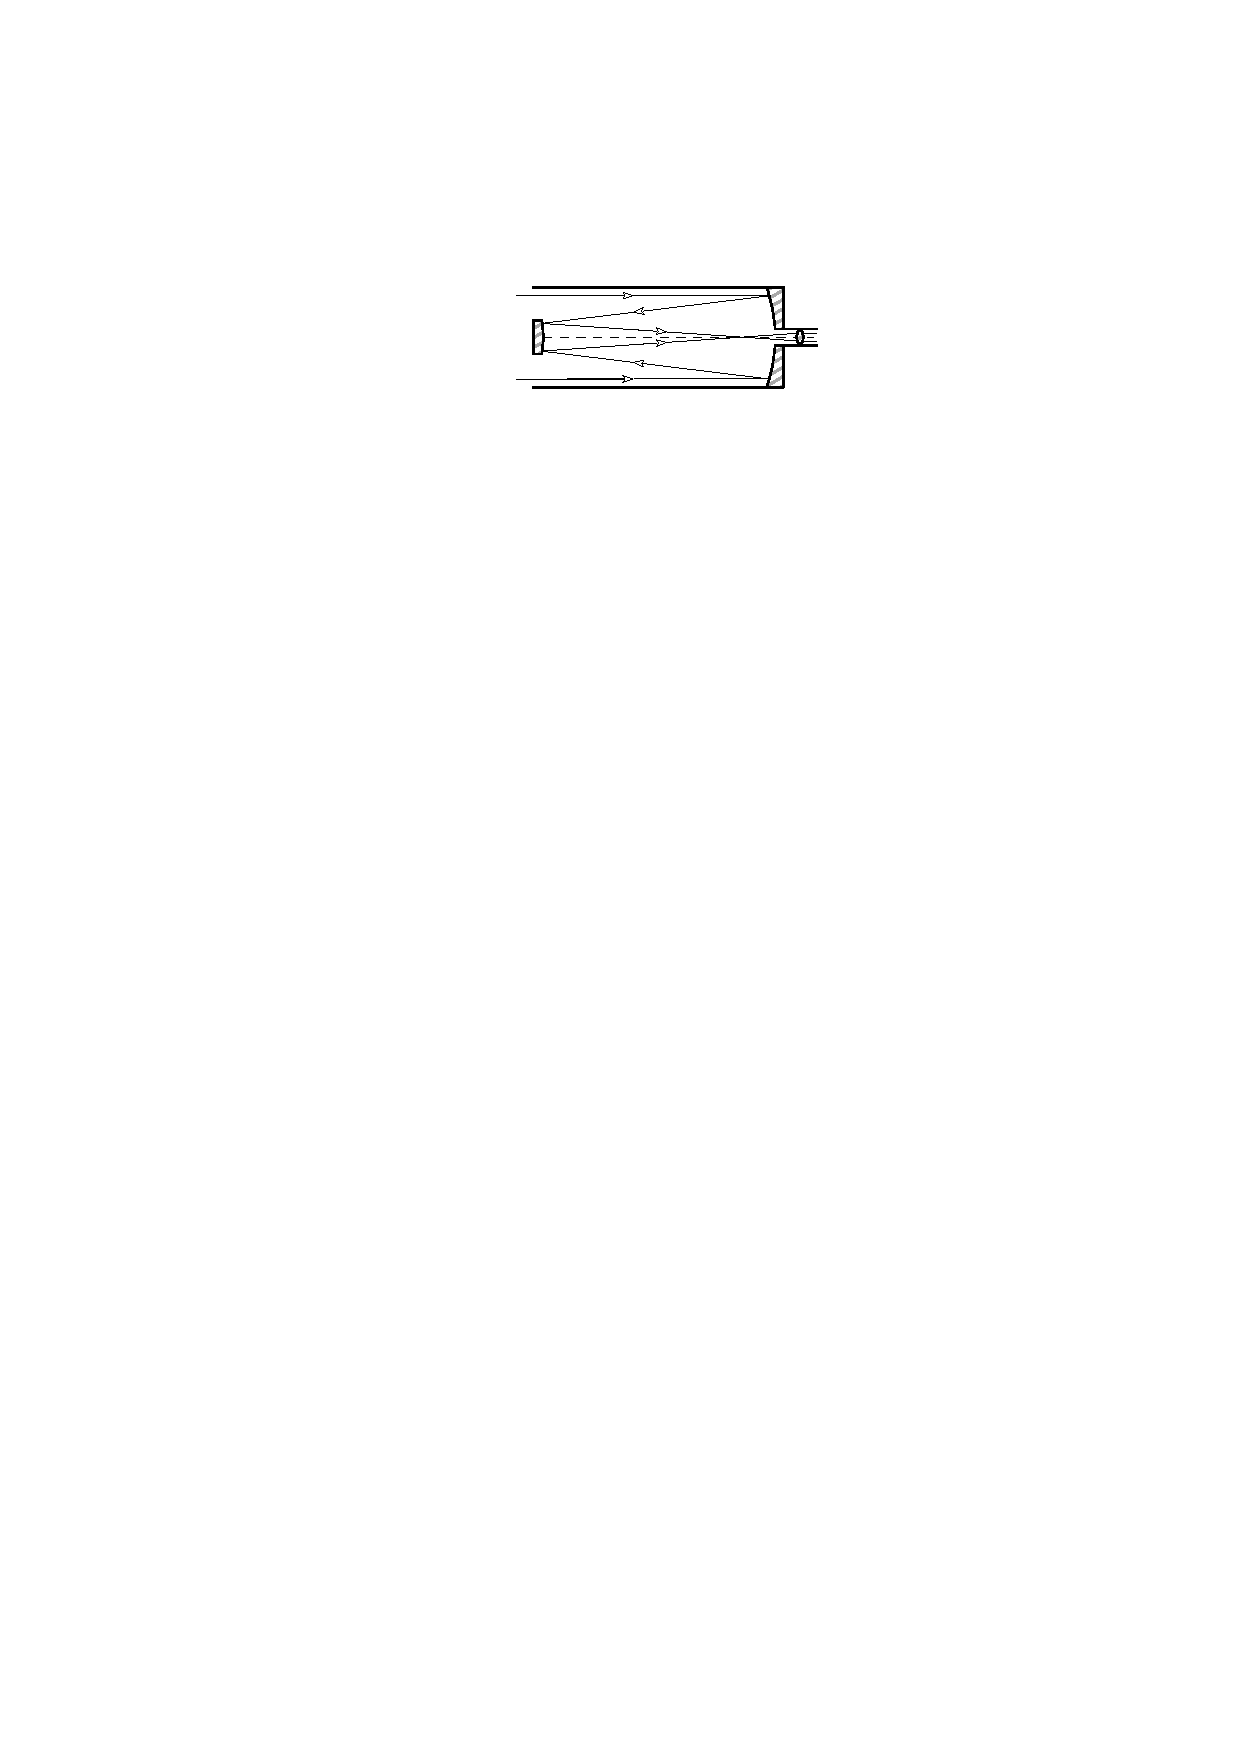
\includegraphics[width = \tw]{Cassigren.pdf}
		\caption{Рефлектор системы Кассегрена}
	\end{subfigure}
	\hfill
	\begin{subfigure}{0.49\tw}
		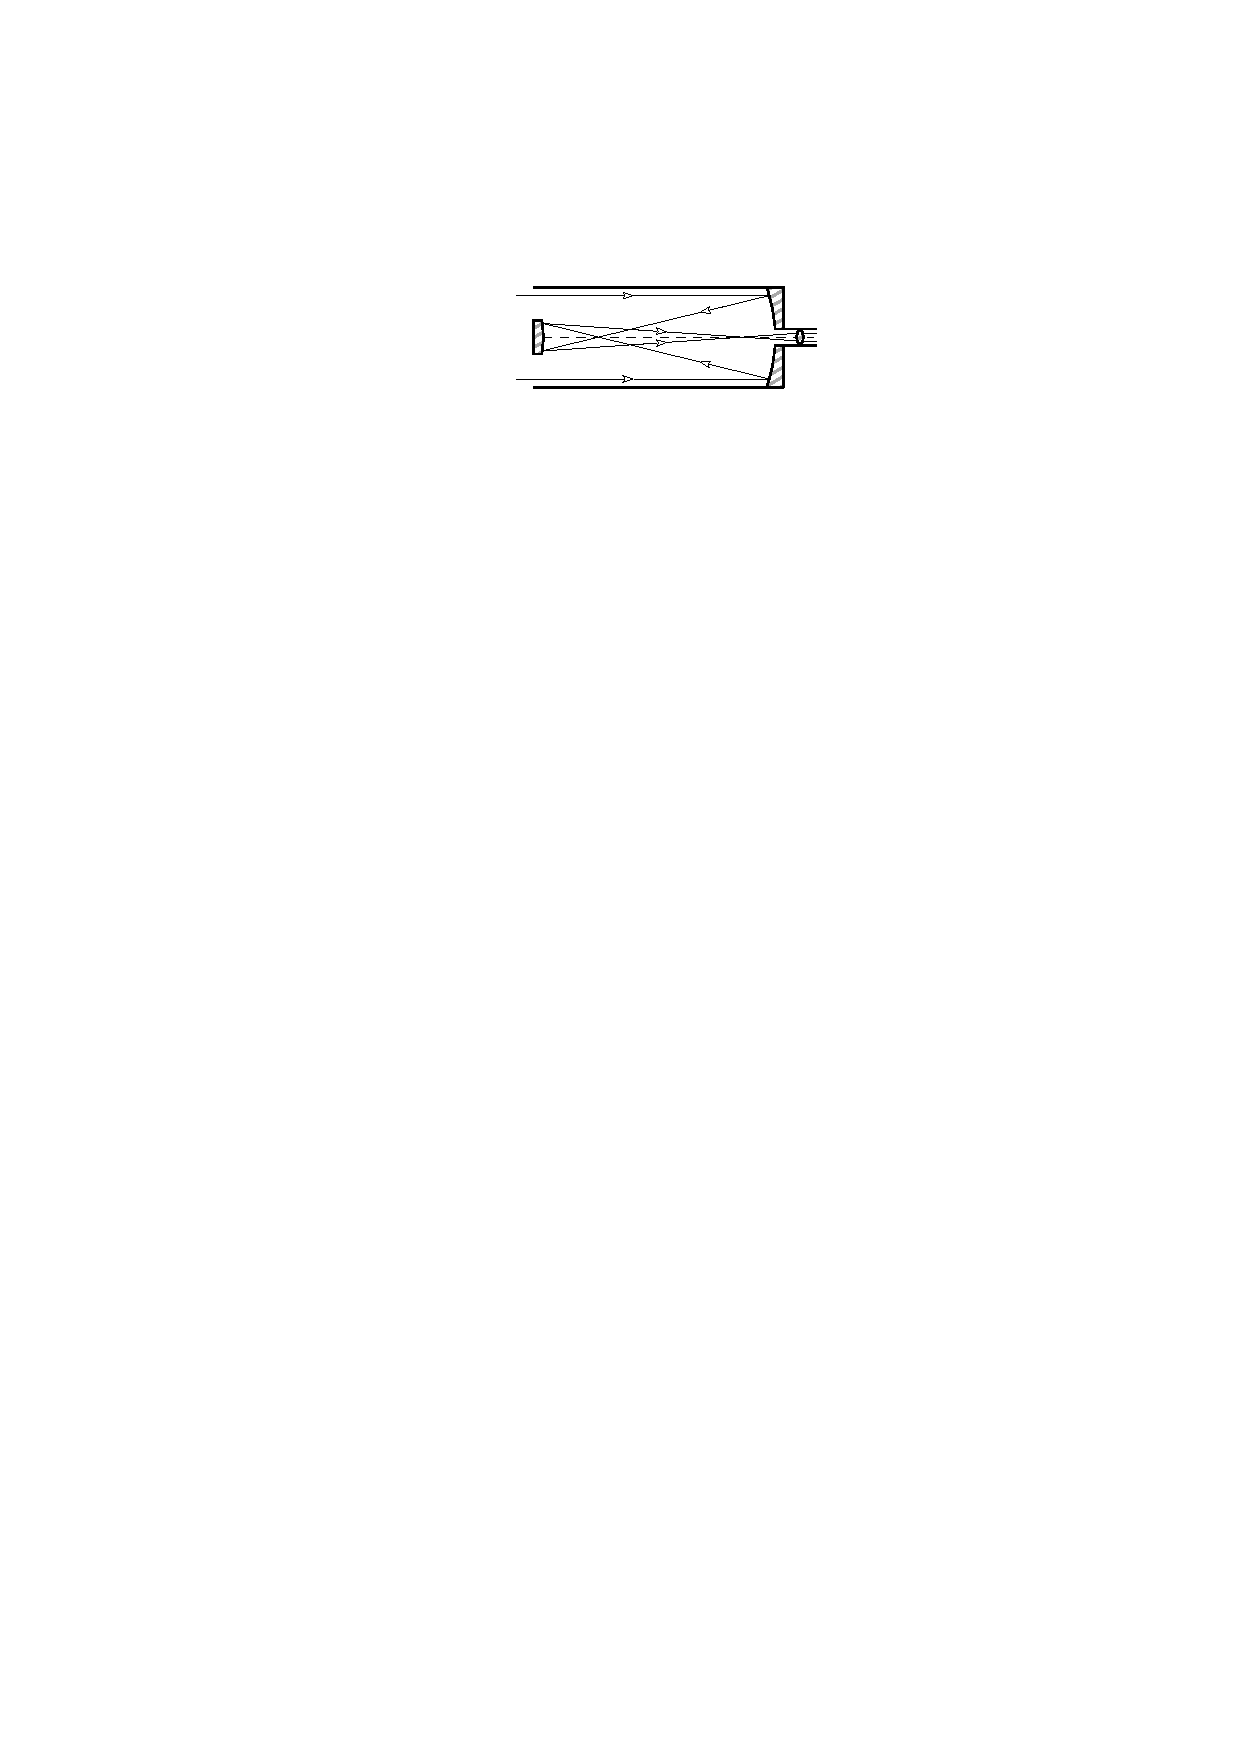
\includegraphics[width = \tw]{Gregory.pdf}
		\caption{Рефлектор системы Грегори}
		\label{Gregory}
	\end{subfigure}
	\vskip4pt
	\begin{subfigure}{0.49\tw}
		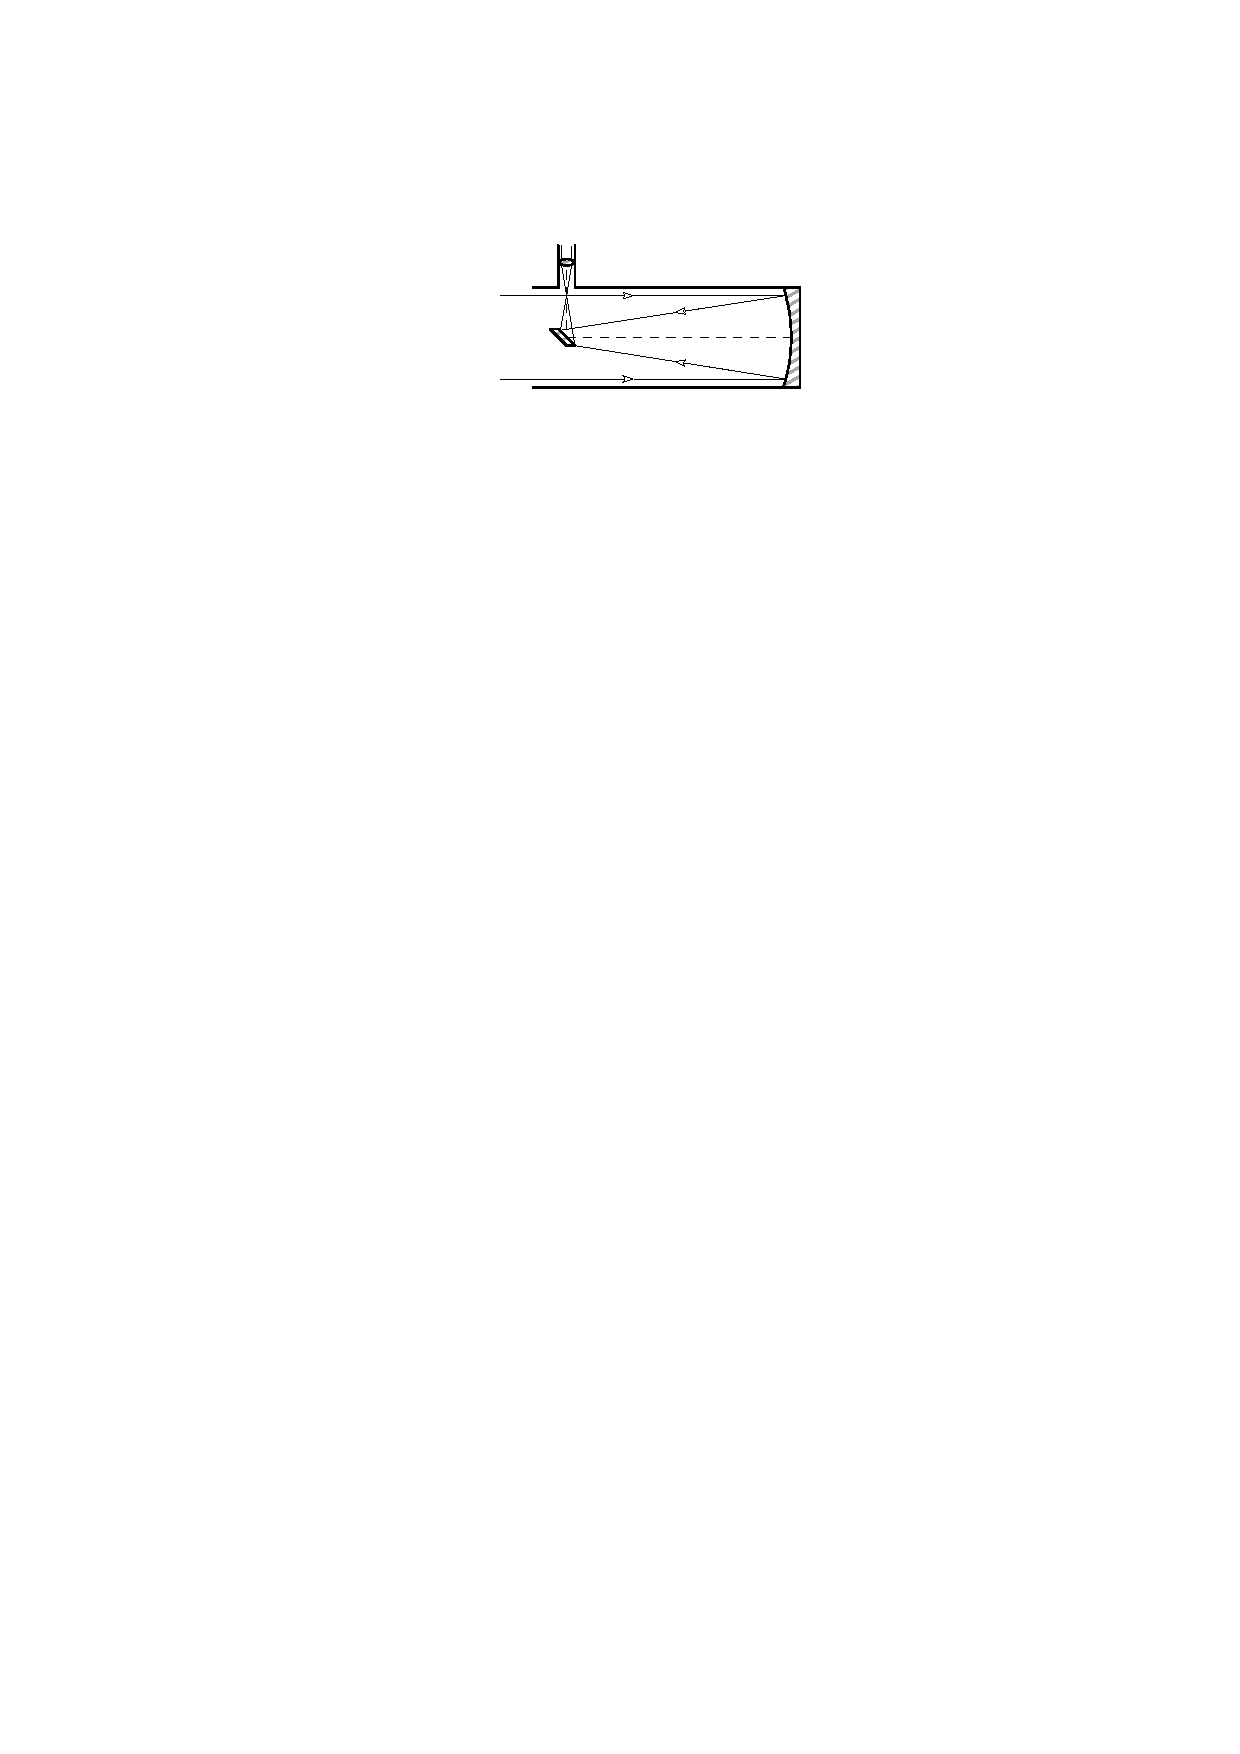
\includegraphics[width = \tw]{Newton}
		\caption{Рефлектор системы Ньютона}
	\end{subfigure}
	\hfill
	\begin{subfigure}{0.49\tw}
		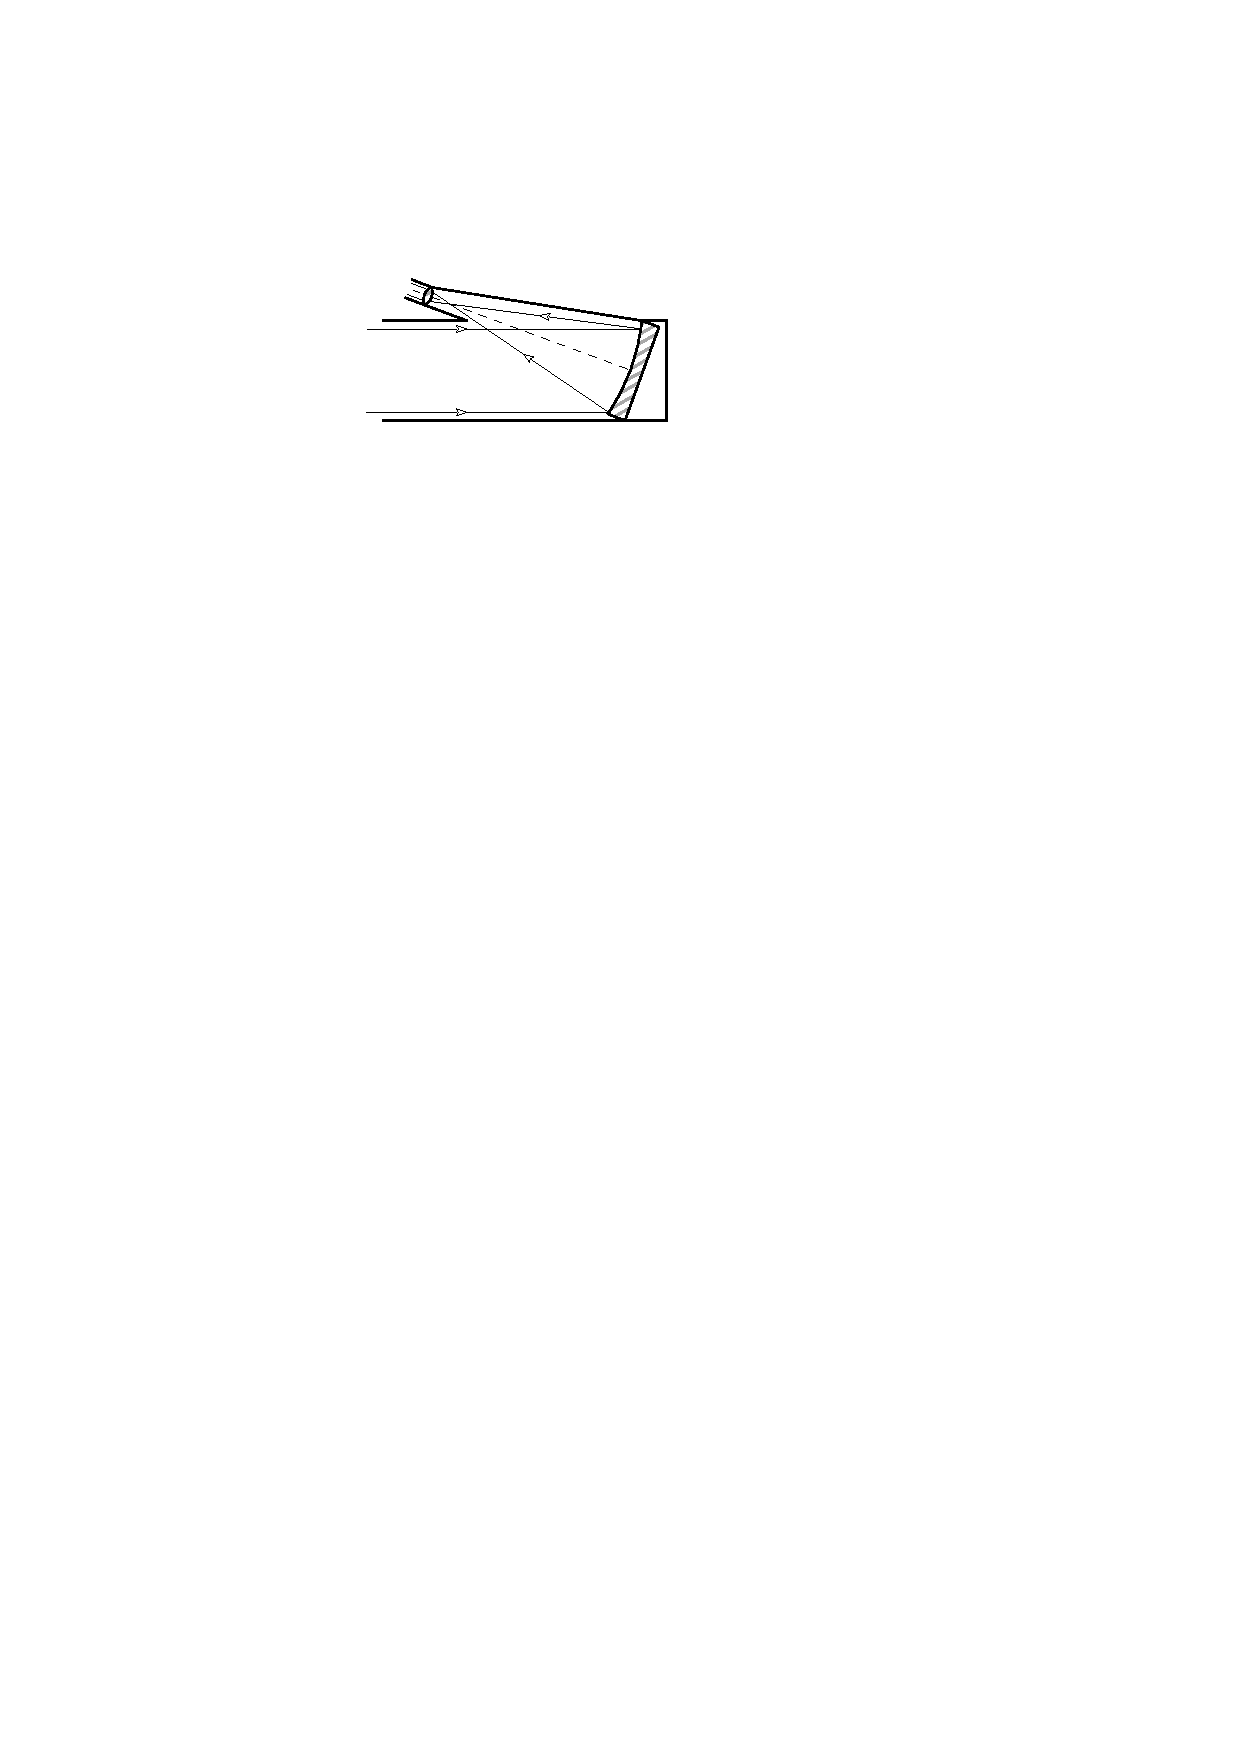
\includegraphics[width = \tw]{Lomonosov.pdf}
		\caption{Рефлектор системы Ломоносова}
	\end{subfigure}
	\caption{Оптические схемы телескопов рефлекторов}
\end{figure}
\term{Рефлектор} (зеркальный телескоп)~---  оптический телескоп,  в котором светособирающими элементами являются зеркала.

\term{Катадиоптрический} (зеркально-линзовый) \term{телескоп}~--- оптический телескоп, в котором используется как система линз, так и зеркал.
